\documentclass[c]{beamer}
                \usepackage{org-preamble}
                \usepackage[cpp_teaching]{slide-style}
                \usepackage{minted}
\usetheme{default}
\title{Compilation et directives de préprocesseur}

\begin{document}

\maketitle

\begin{frame}{Comparaison de quelques langages}
\makebox[\linewidth]{\includegraphics[width=0.8\paperwidth]{langages-perfs.pdf}}
\end{frame}

\begin{frame}{Comparaison de quelques langages}
\makebox[\linewidth]{\includegraphics[width=0.8\paperwidth]{langages-stdlibs.pdf}}
\end{frame}

\begin{frame}{Mécanismes de compilation en C/C++}
\begin{enumerate}
\item \structure{Précompilation :} consiste à traiter, à \emph{parser} les fichiers sources
avant compilation (résolution des directives de préprocesseur
\emph{i.e.} remplacement de macros, suppression de texte, inclusion de
fichiers\ldots{})

\begin{prompt}
g++ -E fichier\_source.cpp
\end{prompt}

{\footnotesize On ne le fait que très rarement soi-même, l'appel du compilateur effectue automatiquement la précompilation.}

\end{enumerate}
\end{frame}

\begin{frame}[fragile]{Mécanismes de compilation en C/C++}
 \begin{enumerate}
\item \structure{Précompilation}
\item \structure{Compilation séparée :} traduction du code en langage machine.
\begin{prompt}
g++ -c fichier\_source.cpp
\end{prompt}
Cette opération conduit à la création d'un \structure{fichier objet} d'extension \texttt{.o}
(ici \texttt{fichier\_source.o}).
\end{enumerate}
\end{frame}

\begin{frame}[fragile]{Mécanismes de compilation en C/C++}
\begin{enumerate}
\item \structure{Précompilation}
\item \structure{Compilation séparée}
\item \structure{Édition de liens :} consiste à regrouper la totalité des données de même que
les fichiers objets et les bibliothèques (fonctions de la bibliothèque
standard et des autres bibliothèques externes) ainsi qu'à résoudre les
références inter-fichiers.
\begin{prompt}
g++ fichier\_source1.o fichier\_source2.o\ldots{} -o~fichier\_executable
\end{prompt}
\end{enumerate}
\end{frame}

%-----------------------------------

\begin{frame}[fragile]{Mécanismes de compilation en C/C++}

\makebox[\linewidth]{\includegraphics[width=0.95\paperwidth]{separate_compilation_linking_1.pdf}}

\end{frame}

\begin{frame}[fragile]{Mécanismes de compilation en C/C++}

\makebox[\linewidth]{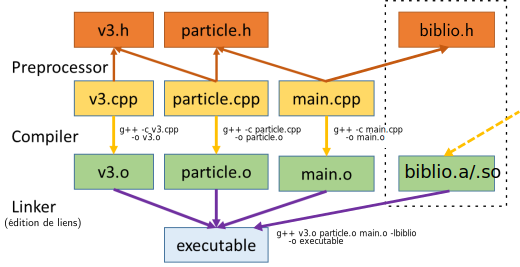
\includegraphics[width=0.95\paperwidth]{separate_compilation_linking_2.pdf}}

\end{frame}

%------------------------------------

\begin{frame}[fragile]{Mécanismes de compilation en C/C++}
\begin{itemize}
\item Les trois précédentes étapes peuvent être réalisées en une seule opération via
la commande

\begin{cbox}
\begin{prompt}
g++ fichier\_source1.cpp fichier\_source2.cpp\ldots{} -o~fichier\_executable
\end{prompt}
\end{cbox}

\begin{cbox}[][][\centering]
\ding{42} Les fichiers d'en-tête ne sont jamais compilés !
\end{cbox}

\item Le binaire ainsi généré \texttt{fichier\_executable} peut alors être exécuté depuis le
répertoire local
\begin{cbox}
\begin{prompt}
./fichier\_executable
\end{prompt}
\end{cbox}

\item À partir du deuxième TD, on proposera aussi l'utilisation d'un \textit{Makefile}

\end{itemize}
\end{frame}

\begin{frame}[fragile,label={sec:orgheadline5}]{Options de compilation}
 \begin{itemize}
\item \structure{l'option \texttt{-Ichemin}} indique au compilateur où sont localisés les fichiers
d'en-têtes nécessaires à la compilation séparée du programme. Par défaut, le
compilateur recherche ces fichiers localement et dans le répertoire
\texttt{/usr/include},
\end{itemize}

\pause

\begin{itemize}
\item \structure{l'option \texttt{-W}} permet l'activation des messages de mise en garde. Différents
niveaux sont accessibles, le plus complet étant \texttt{-Wall -Wextra},
\end{itemize}


\end{frame}

%---------------------------------------------------------

\begin{frame}[fragile]{Démystifier la command \texttt{ccc} (\footnotesize{cf L3 Physique fondamentale, Orsay})}
 \centering
\begin{animateinline}[step,poster=last]{1}
  %%, controls, buttonsize=1em, buttonfg=0.6:0.6:0.6
  \clearbuf\scroll{0.9\linewidth}{8}{\noexpand\$\;which ccc}
  \newframe
  \scroll{0.9\linewidth}{8}{%
    \noexpand\color{orange}/public/mphyo/bin/ccc}
  \newframe
  \scroll{0.9\linewidth}{8}{%
    \noexpand\$\;more /public/mphyo/bin/ccc}
  \newframe
  \scroll{0.9\linewidth}{8}{\noexpand\color{orange}
    g++ -Wall -I/usr/include/python2.7 \textbackslash §§
    \noexpand\color{orange}\hskip +15pt-I/public/mphyo/bibli\noexpand\_fonctions \noexpand\color{green}\$1 \textbackslash §§
    \noexpand\color{orange}\hskip +15pt/public/mphyo/bibli\noexpand\_fonctions/bibli\noexpand\_fonctions.ar \textbackslash §§
    \noexpand\color{orange}\hskip +15pt-lm -lpython2.7 \noexpand\&\& ./a.out \noexpand\color{green}\$1 §§
    \noexpand\color{orange}rm ./a.out 
    
  }
\end{animateinline}
\end{frame}

\begin{frame}[fragile]{Directives de préprocesseur}
 Le préprocesseur recherche des directives de compilation repérées en début de
ligne par le symbole \texttt{\#} et se terminant avec la fin de la ligne

\begin{minted}[fontsize=\footnotesize,samepage,mathescape,xrightmargin=0.5cm,xleftmargin=0.5cm]{c++}
#directive [paramètre]
\end{minted}

On utilise des directives d'inclusion, de définition et de condition. Par exemple,

\begin{minted}[fontsize=\footnotesize,samepage,mathescape,xrightmargin=0.5cm,xleftmargin=0.5cm]{c++}
#include <iostream>
#define PI 3.141592
#if, #ifdef, #ifndef .... #endif  
\end{minted}

Les directives de condition permettent de contrôler ce qui sera compilé effectivement ou non.

\end{frame}


\begin{frame}[fragile,label={sec:orgheadline8}]{Utilisation de directives de condition}
 Il est possible de contrôler ce qui sera compilé effectivement ou non, avec les
clauses de condition :

\begin{minted}[fontsize=\footnotesize,samepage,mathescape,xrightmargin=0.5cm,xleftmargin=0.5cm]{c++}
#if condition
...
#endif
\end{minted}

Le code compris dans la séquence \texttt{\#if} -- \texttt{\#endif} est considéré par le
compilateur seulement si la condition est vraie (non nulle).
\end{frame}

\begin{frame}[fragile,label={sec:orgheadline9}]{Exemple}
 \begin{itemize}
\item \structure{\texttt{test\_debug.cpp}}
\begin{minted}[fontsize=\footnotesize,samepage,mathescape,xrightmargin=0.5cm,xleftmargin=0.5cm]{c++}
#include <iostream>
using namespace std;

int main()
{
#if (DEBUG == 1)
  cout << "DEBUG: "
       << "Mode debug du programme" << endl;
#else
  cout << "NOTICE: "
       << "Mode normal du programme" << endl;
#endif
}
\end{minted}
\end{itemize}

Compilation :
\begin{prompt}
g++ -DDEBUG=1 test\_debug.cpp -o test\_debug
\end{prompt}
\end{frame}


\begin{frame}[<+->][fragile]{Compilation séparée}
 \begin{itemize}
\item \structure{\texttt{dummy.h}}
\begin{minted}[fontsize=\footnotesize,samepage,mathescape,xrightmargin=0.5cm,xleftmargin=0.5cm]{c++}
#ifndef _DUMMY_H_
#define _DUMMY_H_
void dummy();
#endif
\end{minted}

\item \structure{\texttt{dummy.cpp}}
\begin{minted}[fontsize=\footnotesize,samepage,mathescape,xrightmargin=0.5cm,xleftmargin=0.5cm]{c++}
#include "dummy.h"
#include <iostream>
void dummy() { std::cout << "coucou !" << std::endl; }
\end{minted}

\item \structure{\texttt{test\_dummy.cpp}}
\begin{minted}[fontsize=\footnotesize,samepage,mathescape,xrightmargin=0.5cm,xleftmargin=0.5cm]{c++}
#include "dummy.h"
int main() {
  dummy();
}
\end{minted}
\end{itemize}

\pause
Compilation :
\begin{prompt}
g++ dummy.cpp test\_dummy.cpp -o test\_dummy
\end{prompt}
\end{frame}


%------------------------

\begin{frame}[<+->][fragile]{Utilité des fichiers séparés ?}
 \begin{enumerate}
\item \structure{Protection du code source :} un utilisateur \(\lambda\) n'a besoin que de la
déclaration de la fonction \emph{i.e.} le fichier \texttt{dummy.h} et du fichier objet
associé \emph{i.e.} \texttt{dummy.o} (comme dans une bibliothèque).

\item \structure{Temps de compilation :} seuls les fichiers sources \emph{i.e.} \texttt{*.cpp} modifiés,
doivent être recompilés.

\item \structure{Structure/Organisation du code :} à terme chaque structure/classe nouvellement
crée se verra associer deux fichiers, sa déclaration et sa définition, ainsi
qu'un programme \texttt{test}.
\end{enumerate}
\end{frame}


\end{document}
